\RequirePackage[T1]{fontenc}
\documentclass[conference,a4paper]{IEEEtran}
\usepackage{amsmath}
\usepackage{graphicx}
\usepackage{booktabs}
\usepackage{array}
\usepackage{cite}
\usepackage{url}
\usepackage[hidelinks]{hyperref}
\usepackage{pdfpages}
\newcommand{\evidencecite}[3]{\cite[#3]{#2}}
\newcommand{\model}{\texttt{gpt-6.1-sol}}

\title{Equivalent Prompt Formats at a Correctness Ceiling:\\A Bounded Code-Generation Study}
\author{\IEEEauthorblockN{Altan Esmer}
\IEEEauthorblockA{Scientific Methods course project\\
Preliminary draft for author review, 23 October 2026}}

\begin{document}
\maketitle

\begin{abstract}
Prompt sensitivity concerns changes in model behavior when a prompt is varied. A functional-correctness experiment can detect such changes only when its tasks and tests expose differences. This exploratory study compares prose, numbered-list, and XML presentations of equivalent programming requirements. Twelve selected public competition problems were presented twice in each format, producing 72 first responses with the requested model \model{} and medium reasoning. Tasks, prompts, tests, allocation, and analysis were frozen before collection. Isolated generation excluded configured access to local references and tests. Every program passed its retained suite, giving 13,068 successful case checks across 72 programs. All task-level format contrasts and both equal-task mean contrasts were zero. These observations establish a finite-sample correctness ceiling, not statistical equivalence or general prompt insensitivity. The study documents a reproducible comparison and the remaining measurement limits, including public task exposure, small retained inputs, two responses per cell, and incomplete provider observability.
\end{abstract}

\begin{IEEEkeywords}
prompt sensitivity, code generation, prompt formatting, functional correctness, ceiling effect
\end{IEEEkeywords}

\section{Introduction}
When requirements remain the same, a model user may expect presentation choices to leave the quality of generated code unchanged. This expectation is testable, but the answer depends on which prompts, tasks, models, and outcomes are compared. Sclar et al.\ report substantial accuracy differences under formatting variations in their few-shot evaluations of open models \evidencecite{C01}{ICLR2024_6c0e99d7}{p.~1}. That result motivates checking multiple formats; it does not specify the effect expected for a different model or for executable programs.

This paper studies a bounded question: \emph{How do prose, numbered-list, and XML presentations of equivalent programming requirements affect all-case pass rates for \model{} with medium reasoning on twelve selected public programming tasks?} The goal is to describe observed correctness under a fixed intervention. It is not to optimize prompts or to rank models.

The contribution is an auditable comparison with separate collection and grading and explicit reference isolation. All 72 programs passed their retained tests. We report this ceiling without replacing tasks or outcomes after collection, and examine the resulting measurement limits.

\section{Related work}
\subsection{Prompt interventions differ}
Demonstration order is one source of variation. Lu et al.\ show that changing the order of few-shot examples can change classification performance \evidencecite{C02}{lu-etal-2022-fantastically}{p.~8086}. Zhao et al.\ report instability across prompt formats, examples, and their order, and reduce variance with contextual calibration \evidencecite{C08}{pmlr-v139-zhao21c}{PDF p.~1}. Their calibration estimates answer bias in few-shot prediction. It differs from this project's earlier phases called calibration, which screened task difficulty.

Our intervention preserves the ordered requirement blocks and adds no demonstrations. It changes their rendering. Accordingly, evidence about example order provides related context rather than a prediction of the present format contrasts.

\subsection{Sensitivity depends on the outcome}
Hua et al.\ identify heuristic evaluation methods as a contributor to apparent prompt sensitivity in their evaluated natural-language benchmarks \evidencecite{C03}{hua-etal-2025-flaw}{p.~19889}. Their finding motivates separating properties of responses from properties of scoring. It does not establish that every observed prompt effect is an evaluation artifact.

ProSA studies instance-level prompt variation and reports differences across models and datasets \evidencecite{C04}{zhuo-etal-2024-prosa}{p.~1950}. POSIX instead quantifies changes in response log-likelihood under prompt variation \evidencecite{C05}{chatterjee-etal-2024-posix}{p.~14550}. Sheng Lu et al.\ use sensitivity as a proxy for model performance in their evaluated setting \evidencecite{C07}{lu-etal-2024-prompts}{p.~5833}. These operational definitions differ from the all-case functional outcome used here. Different source programs can pass the same fixtures while differing in likelihood, style, efficiency, or behavior on untested inputs.

\subsection{Broader robustness and mitigation}
Qiang et al.\ study input perturbations in intent classification and slot filling and propose prompt perturbation consistency learning \evidencecite{C06}{qiang-etal-2024-prompt}{p.~1357}. Cao et al.\ introduce an evaluation based on semantically equivalent case-level queries \evidencecite{C09}{NEURIPS2024_7fa5a377}{p.~1}. Fu and Barez propose Latent Adversarial Paraphrasing, which optimizes latent perturbations together with model performance \evidencecite{C10}{fu-barez-2025-question}{p.~31305}.

These interventions and outcomes differ from our fixed-renderer comparison of executable correctness. Their results motivate measurement but do not supply a common effect size to pool with our observations.

\section{Data and methods}
\subsection{Task source and preparation}
We used the test split of the BAAI/TACO dataset, whose official record describes code generation from natural-language specifications \evidencecite{C11}{taco-dataset}{dataset card}. The frozen dataset revision is \texttt{d593ed0a2becbbc952230bb89be09189bf1056dc}. The source problems were authored outside this project's AI-assisted task construction. External authorship does not imply that the problems were absent from model training.

The final sample contains six tasks labeled MEDIUM and six labeled HARD by the source. Eligible tasks were ranked deterministically by a seeded hash of their external identifier, with the first six per difficulty retained after the documented filters. The filters required standard input/output, sufficient supplied cases, and a statically admissible Python standard-library reference. They excluded interactive or special-judge behavior, floating-point output comparisons, damaged statements, and insufficient reuse provenance. Difficulty labels provided source-defined diversity; they did not measure difficulty for the target model.

Preparation identified statement and fixture defects. Whole-task replacements followed the recorded ranking and documented rules before target-model observations. One semantic contradiction in task 0778 was proved from its rules before its replacement. For the final twelve tasks, input-domain and expected-output-shape checks retained 2,178 of 2,339 supplied cases and recorded 161 exclusions. Every original case, retained index, exclusion reason, and input/output hash remains available. Expected answers were not rewritten to make references pass. Supplied references passed the retained suites before collection.

This process produces a filtered convenience sample with curated test subsets, not an official TACO benchmark score. No target-model calibration gate selected the final tasks, and mixed outcomes were not required for inclusion.

\subsection{Equivalent format intervention}
The canonical contents comprised four fixed implementation clauses and the original question paragraphs in their original order. Format A separated instruction clauses with blank lines and left the question text unchanged. Format B numbered the clauses and question paragraphs. Format C used instruction and paragraph elements with reversible XML escaping. All three included the same outer \texttt{<problem>} wrapper. Thus A is the prose renderer within a shared wrapper, rather than a prompt containing no markup.

Automated recovery checks reconstructed the same instruction and question contents from all variants. The clauses required Python 3.12, the standard library, stdin/stdout behavior, and runnable source without explanation or Markdown fences. No variant added hints, demonstrations, role instructions, or a reasoning request. Table~\ref{tab:excerpt} shows one actual clause in each format. Syntax and token-length consequences are part of the treatment; their individual effects are not separated.

\begin{table}[t]
\caption{Actual instruction excerpt. The remaining clauses and full problem are omitted here, not in the experiment.}
\label{tab:excerpt}
\centering
\small
\begin{tabular}{@{}l>{\raggedright\arraybackslash}p{0.73\columnwidth}@{}}
\toprule
Format & Rendering of the first clause\\
\midrule
A & \texttt{Solve the programming problem below.}\\
B & \texttt{1. Solve the programming problem below.}\\
C & \texttt{<instruction>Solve the programming problem below.</instruction>}\\
\bottomrule
\end{tabular}
\end{table}

\subsection{Allocation and isolated collection}
The design comprised twelve tasks, three formats, and two fresh responses per task and format. Each of the 24 task/repetition blocks contained A, B, and C once. All six possible format orders occurred four times. Blocks and orders were randomized using schedule seed 20261022 and frozen before dispatch. This seed controls allocation, not model sampling.

The client explicitly requested \model{} with medium reasoning, disabled fallback, and exposed no execution or browsing tools. Every response used a distinct fresh thread. Generation ran in an unprivileged container without repository, reference, test, prior-answer, home-directory, credential, or Docker-socket mounts. The container had no direct external network route; a restricted trusted relay provided its model-service route. Credentials remained outside generation. Offline synthetic checks tested this boundary.

A live preflight on 23 October 2026 used a synthetic marker unrelated to the study tasks and passed before collection. Dispatch records were checked for the frozen prompts and settings. The backend reported the requested model alias. These records do not independently attest to provider weights, model revision, or internal reasoning behavior. Temperature and model sampling seed were not controlled.

The first final answer from each scheduled trial was retained without feedback, repair, follow-up, or answer selection. Collection closed before grading began. All 72 generations completed once in frozen order. Isolation limits configured retrieval of reference artifacts; it cannot remove pretrained knowledge or establish that public tasks are unfamiliar.

\subsection{Execution and analysis}
The primary outcome was whether a returned program passed every retained case for its task. The frozen grader treated the raw answer as Python source, without stripping fences or repairing code. It compared whitespace-separated output tokens exactly, with no numeric tolerance, case folding, or deletion of extra output.

Each case ran in a fresh Python 3.12 container with one CPU, 512 MiB memory, a 64-process limit, read-only code/input mounts, and no network. The ten-second wall limit began after container creation and included start/attach overhead. Standard output and standard error each had a 1 MiB limit. Expected outputs stayed on the host. Program errors and timeouts counted as unsuccessful responses; infrastructure failures and missing responses were separate incomplete outcomes.

Let $Y_{tfr}$ indicate all-case success for task $t$, format $f$, and repetition $r$. For each task and format, the reported rate is
\begin{equation}
\widehat p_{tf}=\frac{Y_{tf1}+Y_{tf2}}{2}.
\end{equation}
The task-level contrasts are $\widehat p_{tB}-\widehat p_{tA}$ and $\widehat p_{tC}-\widehat p_{tA}$. Each mean contrast weights the twelve tasks equally, for example
\begin{equation}
\widehat\Delta_{BA}=\frac{1}{12}\sum_{t=1}^{12}
(\widehat p_{tB}-\widehat p_{tA}).
\end{equation}
The complete-design contrasts required all 72 outcomes to be evaluable. No confirmatory significance or equivalence test was prespecified. Case checks were not treated as independent model responses.

\section{Results}
All scheduled responses had evaluable outcomes. Each program passed every retained case, with no execution or infrastructure errors. Table~\ref{tab:results} reports all task/format cells. Formats A, B, and C each had 24 successes among 24 programs. Every cell was 2/2, every task-level contrast was zero, and both equal-task mean contrasts were zero.

\begin{table}[t]
\caption{All-case successes by task and format. M and H are the dataset difficulty labels. Cases are retained fixtures per program.}
\label{tab:results}
\centering
\small
\begin{tabular}{@{}llrrrr@{}}
\toprule
Task & Label & Cases & A & B & C\\
\midrule
0074 & M & 143 & 2/2 & 2/2 & 2/2\\
0152 & H & 18 & 2/2 & 2/2 & 2/2\\
0250 & M & 254 & 2/2 & 2/2 & 2/2\\
0320 & M & 237 & 2/2 & 2/2 & 2/2\\
0339 & H & 225 & 2/2 & 2/2 & 2/2\\
0402 & M & 179 & 2/2 & 2/2 & 2/2\\
0466 & H & 135 & 2/2 & 2/2 & 2/2\\
0472 & M & 160 & 2/2 & 2/2 & 2/2\\
0581 & H & 205 & 2/2 & 2/2 & 2/2\\
0760 & M & 334 & 2/2 & 2/2 & 2/2\\
0799 & H & 50 & 2/2 & 2/2 & 2/2\\
0979 & H & 238 & 2/2 & 2/2 & 2/2\\
\midrule
Total & & 2,178 & 24/24 & 24/24 & 24/24\\
\bottomrule
\end{tabular}
\end{table}


Across the twelve tasks, 2,178 retained fixtures were applied to six programs per task, yielding 13,068 successful case checks. This count describes repeated checks of 72 programs. It is not a sample of 13,068 independent model outputs.

The collection and grading records bind answers to prompt hashes, thread identifiers, image identities, retained source-case indices, and input/output hashes. Verification confirmed the 196-artifact freeze before grading. A separately scoped reviewer reconciled the saved collection, grading, and analysis records. Review used one model family and supplies artifact checking rather than independent provider attestation.

\section{Discussion and limitations}
\subsection{What the ceiling establishes}
No all-case success difference was observed among the tested renderers, tasks, and first responses. The data provide no preferred format under the finite retained suites and recorded conditions.

The ceiling leaves relative failure probabilities poorly characterized. Equal scores do not establish statistical equivalence, a universally small effect, or general prompt insensitivity. No equivalence margin or power calculation was specified. We report descriptive contrasts without constructing confidence intervals from the case-check count.

External authorship and restricted generation reduce dependence on project-generated contracts and configured local reference access. They do not explain the ceiling. Strong performance, familiar public tasks, limited fixtures, and the chosen intervention remain plausible explanations that this design cannot separate.

\subsection{Validity and generalization}
The twelve tasks are a filtered convenience sample. Standard input/output and reference eligibility exclude other programming work. Two repetitions per cell provide little information about variability. Fresh threads prevent conversational carryover but do not prove independent sampling inside a shared provider service.

Public questions and solutions could have appeared in training. The model's training cutoff, weights, revision, and some sampling settings are unavailable. The observed alias and requested effort are the available configuration evidence; results should not be generalized to all systems using a similar name.

Retained fixtures also cover only part of the declared input space. For example, task 0339 has retained arrays of at most 30 elements despite a statement limit of 500,000. Task 0760 has at most 20 despite a limit of 100,000. Passing these suites does not establish full-constraint correctness or runtime quality. A program with unsuitable asymptotic cost may pass. The frozen study added no large-input stress suite.

Scoring measures exact required output under the saved contract. It does not measure maintainability, explanation quality, likelihood sensitivity, or all semantic properties of the generated programs. References, validators, protocol preparation, and review were AI-assisted within one model family, so correlated errors remain possible. Recorded source-defect checks and independent scopes reduce particular risks without providing a complete correctness proof.

\subsection{Earlier phases and next research}
Two earlier custom-task pilots each produced 45/45 functional passes. A first baseline task calibration produced 18/18, and a composite-task calibration produced 30/30. No family met the qualification rule for the conditional third pilot, which was not launched. A later audit applied stronger tests to the same 30 saved composite answers and produced 4,770/4,770 successful checks without generating new responses. These phases informed this design but used different tasks, interventions, or controls. They are historical context and are not pooled with the present 72 programs.

A future experiment should freeze a fresh task source, failure-exposing tests, a sampling rationale, and an analysis plan before collecting responses. It should establish what effect size matters and preserve the task grouping in its uncertainty analysis. New outcomes found by inspecting these saved answers would be exploratory. They should not replace this study's frozen primary endpoint as confirmatory evidence.

\section{Conclusion}
A separately frozen comparison of three equivalent renderers produced 72/72 all-case successes on twelve selected public tasks. Both mean contrasts were zero. The result is an observed correctness ceiling. It supports an auditable methods account and a narrow descriptive finding while leaving broader prompt sensitivity unresolved.

\section*{AI assistance and reproducibility}
AI assistants contributed to earlier custom tasks, study design, selection and validation tools, prompt renderers, isolation and grading software, model-response collection, result reconciliation, literature searches, and this manuscript draft. The twelve source problem statements were externally authored. That distinction does not make study construction or verification independent of AI assistance.

For this paper, an assistant checked ten proceedings sources, selected evidence passages, assembled highlighted screenshots, and drafted the outline and LaTeX. Separately scoped agents checked source claims, methods, and results within one model family. This is not independent human scholarly review. The author must review the sources, code, conclusions, and final text; this preliminary draft does not assert that this personal review has occurred.

The public repository is \url{https://github.com/AltanEsmer/ScM}. The reported study is in \texttt{studies/format-study1}; its frozen protocol is preserved as written before collection, and completed outcomes are recorded separately. Data-source attribution, original case records, exclusions, raw answers, grading records, and analysis code remain available. Dataset and upstream problem rights remain with their respective owners; reuse notices are preserved in the source directory. The citation appendix supplies evidence for every external citation occurrence in this draft.

\bibliographystyle{IEEEtran}
\bibliography{../references,additional-references}
\label{lastmainpage}

\clearpage
\onecolumn
\section*{Appendix: Citation evidence}
This appendix is separate from the main paper's page count. The main paper, including references, ends on page~\pageref{lastmainpage}. Each citation occurs once. Evidence IDs persist across edits; bracketed numbers match the bibliography in this draft. Publisher article pages are reproduced with locally applied yellow highlights and source provenance. They support the specific cited claims, not broader conclusions about our model. The dataset record is an additional first-party software/data citation and is not counted among the ten peer-reviewed papers.

\begin{center}
\small
\begin{tabular}{llll}
\toprule
Reference & Occurrence & Source & Evidence location\\
\midrule
{[1]} & C01 & Sclar et al., ICLR 2024 & Publisher PDF p.~1\\
{[2]} & C02 & Yao Lu et al., ACL 2022 & Publisher p.~8086\\
{[3]} & C08 & Zhao et al., ICML 2021 & Publisher PDF p.~1\\
{[4]} & C03 & Hua et al., EMNLP 2025 & Publisher p.~19889\\
{[5]} & C04 & Zhuo et al., Findings 2024 & Publisher p.~1950\\
{[6]} & C05 & Chatterjee et al., Findings 2024 & Publisher p.~14550\\
{[7]} & C07 & Sheng Lu et al., NAACL 2024 & Publisher p.~5833\\
{[8]} & C06 & Qiang et al., Findings 2024 & Publisher p.~1357\\
{[9]} & C09 & Cao et al., NeurIPS 2024 & Publisher PDF p.~1\\
{[10]} & C10 & Fu and Barez, EMNLP 2025 & Publisher p.~31305\\
{[11]} & C11 & BAAI/TACO & Official pinned dataset card\\
\bottomrule
\end{tabular}
\end{center}
The following ten article-evidence pages are organized by persistent source ID. Their reference tags identify the bibliography entries even when physical page order differs from citation order. The last evidence page documents the dataset record. Full publisher URLs and exact highlight fragments are also retained in the repository manifests.
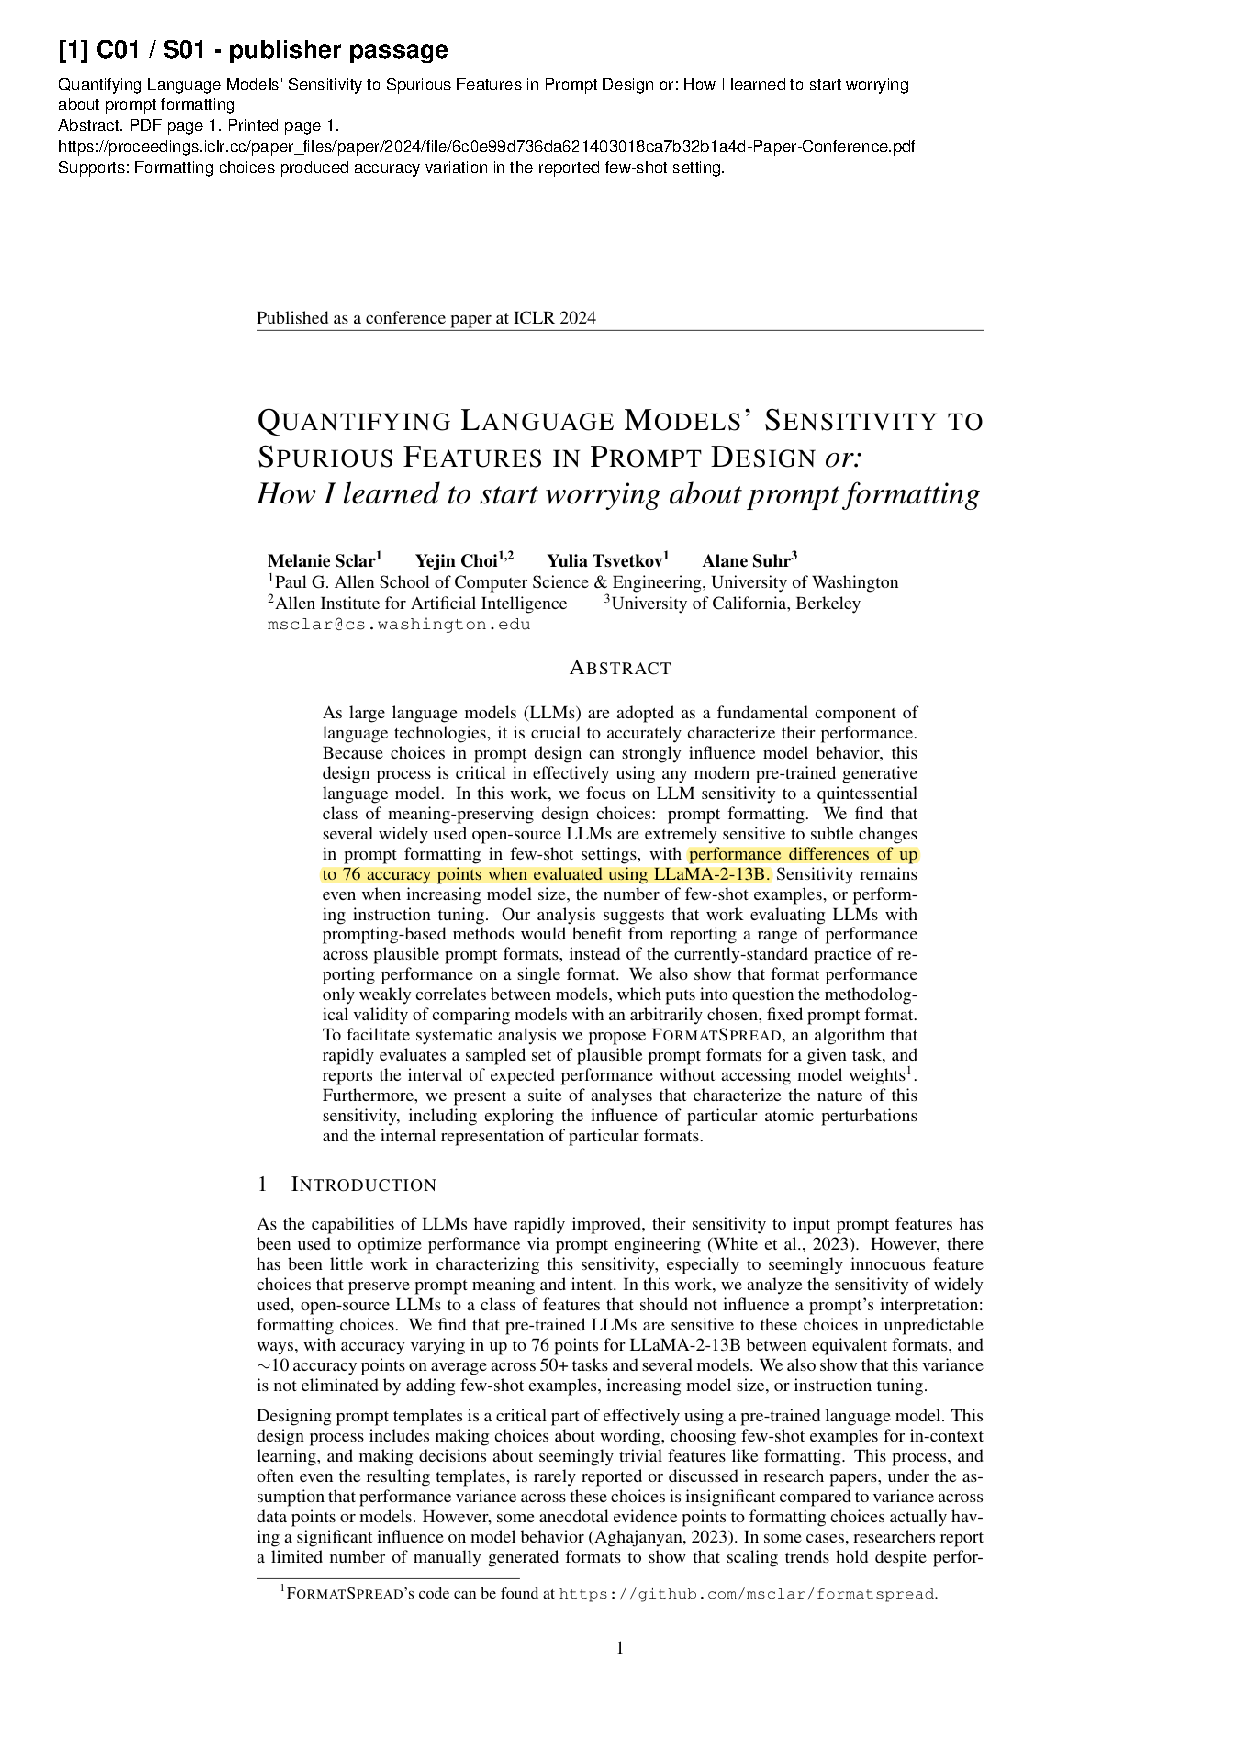
\includepdf[pages=-,pagecommand={\thispagestyle{plain}}]{../output/citation-appendix.pdf}
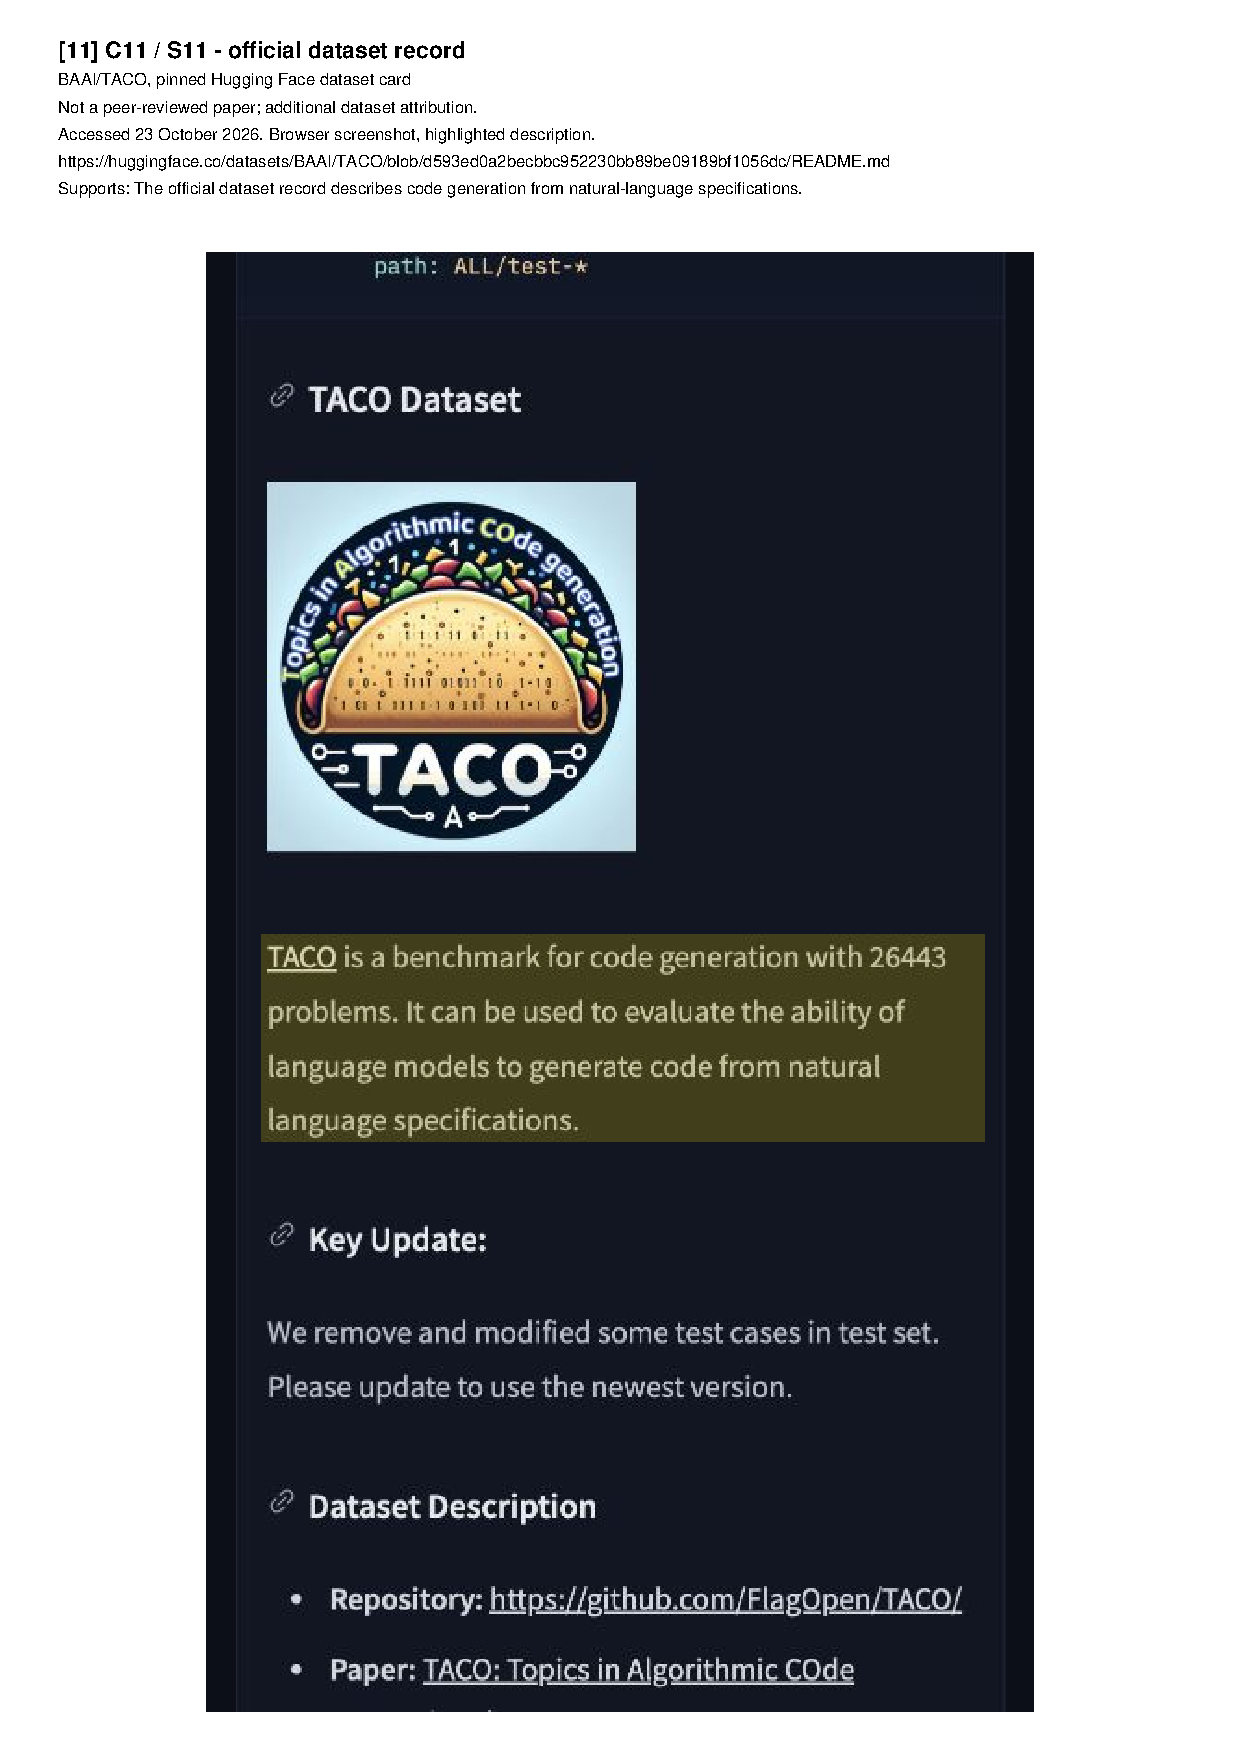
\includepdf[pages=-,pagecommand={\thispagestyle{plain}}]{../evidence/dataset-evidence.pdf}
\end{document}
